\section{Approximated dynamical systems}

\begin{frame}
	\begin{tabular}{l l}
		\begin{minipage}{0.5\textwidth}
			\hspace{-2mm}\paragraph{Linear system:}\vspace{-4mm}
			\begin{itemize}
				\item[$\Rightarrow$] Two dimensional with no parameter
			\end{itemize}%\vspace{-3mm}
			$\dot{x_1} = -0.1 \cdot (x_1 + x_2)$\\
			$\dot{x_2} = 0.25 \cdot x_1$\\
			\vspace{4mm}
			
			\hspace{-2mm}\paragraph{Andronov-Hopf system:}\vspace{-4mm}
			\begin{itemize}
				\item[$\Rightarrow$] Two dimensional with one parameter
			\end{itemize}%\vspace{-3mm}
			$\dot{x_1} = a \cdot x_1 - x_2 - x_1 \cdot (x_1^2 + x_2^2)$\\
			$\dot{x_2} = x_1 + a \cdot x_2 - x_2 \cdot (x_1^2 + x_2^2)$\\
			\vspace{4mm}
			
			\hspace{-2mm}\paragraph{R\"ossler attractor:}\vspace{-4mm}
			\begin{itemize}
				\item[$\Rightarrow$] Three dimensional with one parameter
			\end{itemize}%\vspace{-3mm}
			$\dot{x_1} = -x_2 - x_3$\\
			$\dot{x_2} = x_1 + a \cdot x_2$\\
			$\dot{x_3} = 0.2 + x_3 * (x - 14)$
			\vspace{4mm}
		\end{minipage}
		&
		\begin{minipage}{0.4\textwidth}
			\vspace{-5mm}
			\begin{figure}
				\centering
				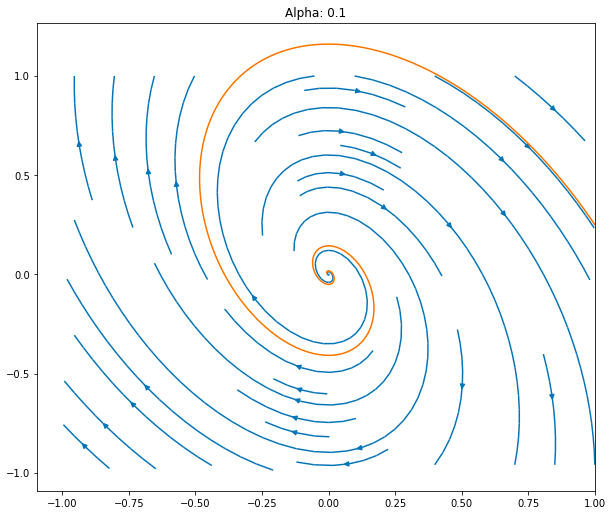
\includegraphics[width=0.6\linewidth]{figures/ls.png}
			\end{figure}\vspace{-4mm}
			\begin{figure}
				\centering
				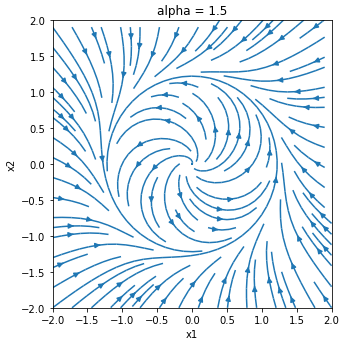
\includegraphics[width=0.5\linewidth]{figures/and_hopf.png}
			\end{figure}\vspace{-4mm}
			\begin{figure}
				\centering
				\hspace{1mm}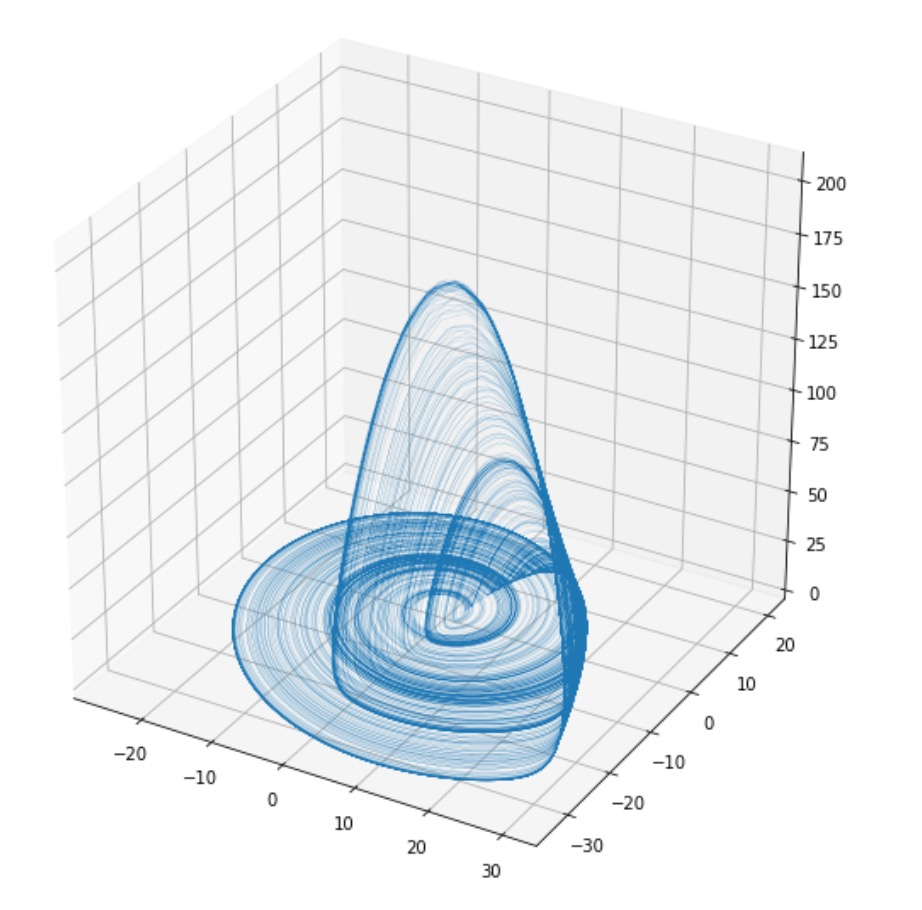
\includegraphics[width=0.6\linewidth]{figures/roe.jpeg}
			\end{figure}
		\end{minipage}
	\end{tabular}
\end{frame}